% !TeX document-id = {4a66a092-a797-425f-b588-c0b0f6bcb4d3}
% !TeX TXS-program:compile = txs:///lualatex/[--shell-escape] | txs:///bibtex | txs:///lualatex/[--shell-escape] | txs:///makeindex | txs:///lualatex/[--shell-escape] | txs:///lualatex/[--shell-escape] | txs:///view
% arara: clean: {
% arara: --> extensions:
% arara: --> ['aux', 'bbl', 'blg', 'idx', 'ilg', 'ind',
% arara: --> 'log', 'out', 'pdf', 'synctex.gz', 'toc']
% arara: --> }
% arara: lualatex
% arara: bibtex
% arara: lualatex
% arara: makeindex
% arara: lualatex
% arara: lualatex: {
% arara: --> shell: yes,
% arara: --> synctex: yes,
% arara: --> interaction: batchmode
% arara: --> }
% arara: clean: {
% arara: --> extensions:
% arara: --> ['aux', 'bbl', 'blg', 'idx', 'ilg', 'ind',
% arara: --> 'log', 'out', 'synctex.gz', 'toc']
% arara: --> }
\RequirePackage{fix-cm}
\documentclass[graybox,envcountchap,sectrefs,a4paper,intlimits]{svmono}
\usepackage{makeidx}         % allows index generation
\usepackage{graphicx}        % standard LaTeX graphics tool
                             % when including figure files
\usepackage{multicol}        % used for the two-column index
\usepackage[bottom]{footmisc}% places footnotes at page bottom
\usepackage{newtxtext}       %
\usepackage[varvw]{newtxmath}% selects Times Roman as basic font
\usepackage{mathtools}
\usepackage{siunitx}

\makeindex             % used for the subject index
                       % please use the style svind.ist with
                       % your makeindex program
\date{4 de julio de 2025}

\usepackage[svgnames]{xcolor}
\usepackage{academicons}
\usepackage[fixed]{fontawesome5}
\usepackage{diffcoeff}
\usepackage{bm}
% https://tex.stackexchange.com/a/556802/117967
\DeclareMathAlphabet{\mathbb}{U}{msb}{m}{n}
% https://tex.stackexchange.com/q/637200
\DeclareMathAlphabet{\mathcal}{OMS}{cmsy}{m}{n}
\newcommand{\MVAt}{{\usefont{U}{mvs}{m}{n}\symbol{`@}}}
\definecolor{orcidcolor}{HTML}{a5ca3f}
\definecolor{orcidlinkcolor}{HTML}{0961ba}

\difdef{c}{L}{op-symbol=\mathop{}\!\mathbin\bigtriangleup}
\difdef{f}{}{outer-Ldelim=\left .,outer-Rdelim=\right |,sub-nudge=0 mu}

\usepackage{hyperref}
\hypersetup{
	pdfencoding=auto,
	linktocpage=true,
	colorlinks=true,
	linkcolor=DarkBlue,
    citecolor=DarkBlue,
	urlcolor=orcidlinkcolor,
	pdfpagelabels,
	pdftex,
	pdfauthor={Carlos Aznarán Laos},
	pdftitle={El Método de Volúmenes Finitos},
	pdfsubject={Proyecto de Tesis II},
	pdfkeywords={fvm, pde},
	pdfproducer={LuaHBTeX, Version 1.22.0 (TeX Live 2026/dev/Arch Linux)},
	% bookmark=false
}
\begin{document}

\author{Carlos Aznarán Laos}
\title{El Método de Volúmenes Finitos}
\subtitle{Proyecto de Tesis II presentado a la \\
    Universidad Nacional de Ingeniería, \\
    Lima, Perú}
\maketitle

\clearpage
\thispagestyle{empty}

\begin{minipage}[t]{0.5\textwidth}
    \textit{Autor} \\
    Carlos Aznarán Laos~\href{https://orcid.org/0000-0001-8314-2271}{\textcolor{orcidcolor}{\aiOrcid}} \\
    Facultad de Ciencias \\
    Universidad Nacional de Ingeniería \\
    Av. Túpac Amaru N$^{\circ}210$ Rímac \\
    Lima 15032, República del Perú \\
    \textcolor{black}{\faIcon{inbox}}
    \href{mailto:caznaranl@uni.pe}{\texttt{caznaranl\MVAt uni.pe}}
\end{minipage}\hfill
\begin{minipage}[t]{0.5\textwidth}
    \textit{Supervisor} \\
    Fidel Jara Huanca~\href{https://orcid.org/0009-0000-1884-1949}{\textcolor{orcidcolor}{\aiOrcid}} \\
    Profesor de la Facultad de Ciencias \\
    Universidad Nacional de Ingeniería \\
    Av. Túpac Amaru N$^{\circ}210$ Rímac \\
    Lima 15032, República del Perú \\
    \textcolor{black}{\faIcon{inbox}}
    \href{mailto:fjarah@uni.edu.pe}{\texttt{fjarah\MVAt uni.edu.pe}}
\end{minipage}

\vfill

% \noindent
% ISSN 2190-5053 \hfill e-ISSN 2190-5061 \\
% ISBN 978-1-4419-7600-0 \hfill e-ISBN 978-1-4419-7601-7 \\
% DOI \href{https://www.doi.org/10.1007/978-1-4419-7601-7}{10.1007/978-1-4419-7601-7}

% \vspace{1cm}

\noindent

\includegraphics[width=.25\textwidth]{CC-BY-NC-SA-4.0} \\
Reconocimiento - No Comercial - Compartir Igual - Sin restricciones adicionales \\
\url{https://creativecommons.org/licenses/by-nc-sa/4.0} \\

\noindent
Usted puede copiar, redistribuir y adaptar este material en cualquier
formato o medio, así como crear obras derivadas a partir de él,
siempre que:

\begin{itemize}
    \item

          Reconozca adecuadamente la autoría original, incluyendo un
          enlace a la licencia e indicando si se realizaron
          modificaciones.

    \item

          No lo utilice con fines comerciales.

    \item

          Comparta cualquier obra derivada bajo la misma licencia.

    \item

          No añada restricciones adicionales que limiten los derechos
          otorgados por esta \linebreak licencia.
\end{itemize}

\frontmatter


%%%%%%%%%%%%%%%%%%%%%%% dedic.tex %%%%%%%%%%%%%%%%%%%%%%%%%%%%%%%%%
%
% sample dedication
%
% Use this file as a template for your own input.
%
%%%%%%%%%%%%%%%%%%%%%%%% Springer %%%%%%%%%%%%%%%%%%%%%%%%%%

\begin{dedication}\index{dedication}
    Dedico este proyecto de tesis II a Dios, a mis queridos padres
    y a mi gran mentor Fidel Jara.
\end{dedication}
%%%%%%%%%%%%%%%%%%%%%%foreword.tex%%%%%%%%%%%%%%%%%%%%%%%%%%%%%%%%%
% sample foreword
%
% Use this file as a template for your own input.
%
%%%%%%%%%%%%%%%%%%%%%%%% Springer %%%%%%%%%%%%%%%%%%%%%%%%%%

\foreword

El presente trabajo titulado
\emph{El Método de los Volúmenes Finitos: Fundamentos y Aplicaciones},
representa un esfuerzo riguroso y detallado por parte del estudiante
en el campo de la discretización numérica de las ecuaciones
diferenciales parciales (EDPs).
A lo largo de esta investigación, se aborda con claridad y
profundidad la formulación matemática del método de volúmenes finitos
(MVF), su implementación práctica y su aplicación a problemas
clásicos, como la ecuación de Poisson y la ecuación de transporte
unidimensional.
Uno de los aspectos más valiosos de esta tesis es la exposición
pedagógica de las aproximaciones de derivadas en las interfaces de
las celdas, respaldada por expansiones de Taylor y un manejo
cuidadoso de las condiciones de frontera.
Asimismo, la discusión sobre esquemas lineales para la ecuación de
transporte y la extensión a leyes de conservación bidimensionales
refleja una visión amplia y aplicada del tema.
Como supervisor, he sido testigo del compromiso y la dedicación del
estudiante en la elaboración de este trabajo.
Su capacidad para conectar teoría, análisis numérico y aplicaciones
prácticas es notable, y estoy convencido de que este documento será
un recurso valioso tanto para estudiantes como para investigadores
que incursionen en el estudio de métodos numéricos para EDPs.

Finalmente, invito al lector a apreciar no solo los resultados
técnicos aquí presentados, sino también el rigor con el que se ha
estructurado cada capítulo, equilibrando formalismo matemático con
intuición física.
Esta tesis no solo cumple con los estándares académicos esperados,
sino que también sienta las bases para futuras investigaciones en el
área\index{foreword}.

\vspace{\baselineskip}
\begin{flushright}\noindent
	Lima, Perú\hfill Prof. Fidel Jara Huanca\\
	julio 2025\hfill {\it\phantom{.}}
\end{flushright}



\preface

Este trabajo nace de mi fascinación por los métodos numéricos y su
poder para transformar ecuaciones diferenciales complejas en problemas
abordables mediante algoritmos computacionales.
El método de volúmenes finitos (MVF) capturó especialmente mi interés
por su elegancia matemática y su capacidad para preservar leyes de
conservación fundamentales en física e ingeniería.
A lo largo de estas páginas, he buscado construir un puente entre la
teoría y la práctica.
Comenzando con los fundamentos del MVF para la ecuación de Poisson
unidimensional, el texto avanza hacia problemas más desafiantes, como
la ecuación de transporte y sistemas bidimensionales.
Cada capítulo refleja horas de estudio, pruebas numéricas y
discusiones valiosas con mi supervisor y colegas, quienes me ayudaron
a refinar mis ideas y corregir errores.

Este documento no pretende ser exhaustivo, sino más bien una guía
accesible para estudiantes que, como yo, inician su camino en el
análisis numérico.
He incluido deducciones detalladas de las aproximaciones clave
—como las derivadas en las interfaces de las celdas— porque hubiera
deseado encontrar explicaciones así de claras cuando comencé a
aprender estos temas.

Agradezco profundamente a mi supervisor, Fidel Jara Huanca, por su
paciencia y orientación; a mis compañeros de laboratorio, por sus
críticas constructivas; y a mi familia, por su apoyo incondicional
durante este proceso.
Invito al lector a abordar este texto con lápiz y papel en mano: los
conceptos se asimilan mejor cuando se recrean paso a paso.
Los errores que persistan son, por supuesto, de mi entera
responsabilidad\index{preface}.

\vspace{\baselineskip}
\begin{flushright}\noindent
	Lima, Perú\hfill Carlos Aznarán Laos
\end{flushright}



%%%%%%%%%%%%%%%%%%%%%%acknow.tex%%%%%%%%%%%%%%%%%%%%%%%%%%%%%%%%%%%%%%%%%
% sample acknowledgement chapter
%
% Use this file as a template for your own input.
%
%%%%%%%%%%%%%%%%%%%%%%%% Springer %%%%%%%%%%%%%%%%%%%%%%%%%%

\extrachap{Agradecimientos}

Quisiera agradecer sinceramente a mi supervisor, el profesor Fidel
Jara Huanca, por su dedicada guía en mi investigación desde cero.
Su talento y espíritu me han inspirado y me han impulsado en mi
camino hacia la ciencia.
El profesor Jara también me ayudó con entusiasmo en mi vida diaria,
prestó gran atención a mi desarrollo profesional y fue un ejemplo
excepcional para mí.
Sin su ayuda y guía, este libro no podría terminarse.

Finalmente, quisiera agradecer sinceramente a toda mi familia por su
continuo y gran apoyo en mi carrera investigadora.


% %%%%%%%%%%%%%%%%%%%%%%acknow.tex%%%%%%%%%%%%%%%%%%%%%%%%%%%%%%%%%%%%%%%%%
% sample declarations chapter
%
% Use this file as a template for your own input.
%
%%%%%%%%%%%%%%%%%%%%%%%% Springer %%%%%%%%%%%%%%%%%%%%%%%%%%

\extrachap{Declaraciones}

\ethics{Conflicto de Intereses}{Please declare any competing interests
    in the context of your chapter. The following sentences can be regarded as examples.\newline
    This study was funded by [X] [grant number X].\newline
    [Author A] has a received research grant from [Company W].\newline
    [Author B] has received a speaker honorarium from [Company X] and owns stock in [Company~Y].\newline 
    [Author C] is a member of [committee Z].\newline 
    The authors have no conflicts of interest to declare that are relevant to the content of this chapter.}

\ethics{Aprobación Ética}{If your chapter includes primary studies with humans please declare the adherence of ethical standards. Example text: This study was performed in line with the principles of the Declaration of Helsinki. Approval was granted by the Ethics Committee of University B (Date.../No. ...).\newline
    In addition, for human participants, authors are required to include a statement that informed consent (to participate and/or to publish) was obtained from individual participants or parents/guardians if the participant is minor or incapable.\newline
    If animals are studied, authors should make sure that the legal requirements or guidelines in the country and/or state or province for the care and use of animals have been followed or specify that no ethics approval was required.}


\tableofcontents
% %%%%%%%%%%%%%%%%%%%%%%acronym.tex%%%%%%%%%%%%%%%%%%%%%%%%%%%%%%%%%%%%%%%%%
% sample list of acronyms
%
% Use this file as a template for your own input.
%
%%%%%%%%%%%%%%%%%%%%%%%% Springer %%%%%%%%%%%%%%%%%%%%%%%%%%

\extrachap{Acrónimos}

Use the template \emph{acronym.tex} together with the document class SVMono (monograph-type books) or SVMult (edited books) to style your list(s) of abbreviations or symbols.

Lists of abbreviations\index{acronyms, list of}, symbols\index{symbols, list of} and the like are easily formatted with the help of the Springer-enhanced \verb|description| environment.

\begin{description}[CABR]
\item[ABC]{Spelled-out abbreviation and definition}
\end{description}

\mainmatter
%%%%%%%%%%%%%%%%%%%%%part.tex%%%%%%%%%%%%%%%%%%%%%%%%%%%%%%%%%%
% 
% sample part title
%
% Use this file as a template for your own input.
%
%%%%%%%%%%%%%%%%%%%%%%%% Springer %%%%%%%%%%%%%%%%%%%%%%%%%%

\begin{partbacktext}
\part{Part Title}
\noindent Use the template \emph{part.tex} together with the document class SVMono (monograph-type books) or SVMult (edited books) to style your part title page and, if desired, a short introductory text (maximum one page) on its verso page.

\end{partbacktext}
\motto{
	Por tanto, estudiantes estudien matemáticas y no construyan sin fundamentos.
	\begin{flushright}\normalfont
		Leonardo da Vinci (1452-1519)
	\end{flushright}
}
\chapter{Motivación}
\label{intro}
% use \chaptermark{}
% to alter or adjust the chapter heading in the running head

\abstract{
	Este capítulo inicia nuestro estudio de las Leyes de Conservación y
	resume el estado del arte de los avances~\cite{Mishra2020} en este
	fascinante campo de las EDPs.
	El principal objetivo es ilustrar las dificultades tanto analíticas
	como numéricas al resolver un \emph{problema de Cauchy} con una
	condición inicial discontinua, soluciones de este tipo no son
	satisfechas en todo punto de su dominio en el sentido clásico, ya
	que las derivadas no son definidas en las discontinuidades.
	Para encontrar la definición correcta, necesitamos entender el
	significado de la forma diferencial de las ecuaciones desde el
	enfoque físico.
	Esto nos llevará al estudio de la forma integral de estas
	ecuaciones y será justificado en este capítulo.
	Además, presentamos diferentes modelos de leyes de conservación que
	nos resume su amplio rango de aplicaciones.
}

\section{Introducción}

Considere un dominio $\Omega\subset\mathbb{R}^{n}$ y una cantidad de
interés $\bm{U}$ definida para todos los $\bm{x}\in\Omega$.
La cantidad de interés podría ser la concentración de un químico o la
densidad de una población humana, la presión de un fluido o la
temperatura de una cuerda.

La evolución en tiempo de esta cantidad de interés $\bm{U}$
puede ser descrito mediante la observación:
\begin{quote}
	La tasa temporal de cambio de $\bm{U}$ en cualquier subdominio
	fijo $\omega\in\Omega$ es igual a la cantidad total de
	$\bm{U}$ producido o destruido dentro de $\omega$ y el flujo
	de $\bm{U}$ a través de la frontera $\partial\omega$.
\end{quote}
Esta observación se describe matemáticamente como
\begin{equation}\label{eq:integralbalance}
	\diff{}{t}
	\int_{\omega}
	\bm{U}\dl{\bm{x}}=
	-\int_{\partial\omega}
	\bm{F}\cdot\nu\dl{\sigma\left(\bm{x}\right)}+
	\int_{\omega}
	\bm{S}\dl{\bm{x}}.
\end{equation}
donde $\nu$ es la normal unitaria exterior,
$\dl{\sigma\left(\bm{x}\right)}$ es la medida de la superficie,
$\bm{F}$ es el flujo y $\bm{S}$ es la fuente.
Así,~\eqref{eq:integralbalance} es la ecuación integral para la
evolución de la cantidad total de $\bm{U}$ en $\omega$.
\begin{figure}[b]
	\sidecaption
	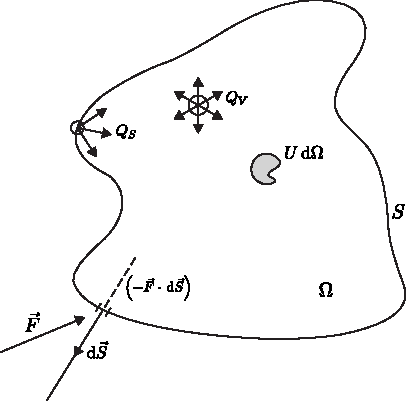
\includegraphics{conservationscheme}
	% If not, use
	%\picplace{5cm}{2cm} % Give the correct figure height and width in cm
	%
	\caption{If the width of the figure is less than 7.8 cm use the
		\texttt{sidecapion} command to flush the caption on the left side of the page.
		If the figure is positioned at the top of the page, align the sidecaption with
		the top of the figure -- to achieve this you simply need to use the optional
		argument \texttt{[t]} with the \texttt{sidecaption} command}
	\label{fig:1}       % Give a unique label
\end{figure}
Simplificamos~\eqref{eq:integralbalance} utilizando el teorema de la
divergencia de Gauß en la integral de superficie para obtener
\begin{equation}\label{eq:integralbalance2}
	\diff{}{t}
	\int_{\omega}
	\bm{U}\dl{\bm{x}}
	+\int_{\omega}
	\operatorname{div}
	\left(\bm{F}\right)\dl{\bm{x}}=
	\int_{\omega}
	\bm{S}\dl{\bm{x}}.
\end{equation}
Dado que~\eqref{eq:integralbalance2} se cumple para cualquier
subdominio $\omega\subset\Omega$,
\begin{equation}\label{eq:balancelaw}
	\forall\left(x,t\right)\in\Omega\times\mathbb{R}_{+}:
	\difcp{\bm{U}}{t}+
	\operatorname{\operatorname{div}
		\left(\bm{F}\right)}=
	\bm{S}.
\end{equation}
La ecuación~\eqref{eq:balancelaw} se llama \emph{ley de balance}.
Frequentemente, el único cambio en $\bm{U}$ proviene de los
flujos y la fuente se fija en cero.
\begin{equation}\label{eq:conservationlaw}
	\forall\left(x,t\right)\in
	\Omega\times\mathbb{R}_{+}:
	\difcp{\bm{U}}{t}+
	\operatorname{\operatorname{div}
		\left(\bm{F}\right)}=
	0.
\end{equation}
La ecuación~\eqref{eq:conservationlaw} se llama
\emph{ley de conservación}, ya que el único cambio en $\bm{U}$
procede de la cantidad que entra o sale del dominio de interés.

\section*{Ejemplos de leyes de conservación}

Algunos ejemplos de leyes de conservación son la ecuación de
transporte escalar, la ecuación de difusión, las ecuaciones de Euler,
la ecuación de Richards y la ecuación Buckley-Leverett.

\subsection*{Ecuación de transporte escalar}

Sea $\bm{U}=U$ la concentración de un contaminante en un río.
Suponga que el río fluye con un campo de velocidad
$\bm{a}\left(\bm{x},t\right)$ y conocemos el campo de
velocidad en todos los puntos del río.
El contaminante es transportado en la dirección de la velocidad, y
así el flujo es $\bm{F}=\bm{a}U$.
Dado que no hay producción ni destrucción del contaminante durante el
flujo, el término fuente en~\eqref{eq:balancelaw} es cero.
La ley de conservación~\eqref{eq:conservationlaw} resulta ser
\begin{equation}
	\difcp{U}{t}+
	\operatorname{div}
	\left(\bm{a}\left(\bm{x},t\right)U\right)=
	0.
\end{equation}

\subsection*{Ecuación de difusión}

Sea $\bm{U}=U$ la temperatura de un bloque metálico.
Suponga que el bloque se calienta por un extremo y se deja enfriar
después, sin aportar ninguna fuente de calor adicional.
El calor se propaga o difunde y la temperatura del bloque se
uniformiza al cabo de un tiempo.
La difusión del calor se rige por la ley de Fick
\begin{equation}\label{eq:ficklaw}
	\bm{F}\left(U\right)=
	-\bm{k}\nabla U.
\end{equation}
Aquí, $\bm{k}$ es el tensor de conductividad del medio.
Sustituyendo~\eqref{eq:ficklaw} en~\eqref{eq:conservationlaw}
resulta ser
\begin{equation*}
	\difcp{U}{t}-
	\operatorname{div}
	\left(\bm{k}\nabla U\right)=
	0.
\end{equation*}

\subsection*{Ecuaciones de Euler}

El aire consiste de un gran número de moléculas.
El movimiento de cada molécula puede seguirse individualmente y
da lugar a un gran número de EDOs.
El sistema EDO resultante es demasiado grande para ser
computacionalmente viable.
En su lugar, se utiliza una descripción macroscópica.
Las variables de interés son: la densidad $\rho$, el campo de
velocidad $u$ y la presión del gas $p$.

\begin{description}
	\item[Conservación de la masa]

	      La masa total de un gas es conservado, garantizado
	      por el Teorema de la circulación de Kelvin.

	\item[Conservación del momento]

	      Se sigue de la segunda ley de Newton que la tasa de cambio de
	      la cantidad de movimiento es igual a la fuerza aplicada.
	      En ausencia de fuerzas externas, la presión del gas es la
	      única fuerza que actúa sobre el gas.

	\item[Conservación de la energía]

	      La energía total de un gas es la suma de su energía cinética
	      y su energía interna (potencial)
\end{description}

\begin{align}
	\difcp{\rho}{t}+
	\operatorname{div}
	\left(\rho\bm{u}\right)                       & =
	0.                                                \\
	\difcp{\rho\bm{u}}{t}+
	\operatorname{div}
	\left(\rho\bm{u}\otimes\bm{u}\right)+\nabla p & =
	0.                                                \\
	\difcp{E}{t}+
	\operatorname{div}
	\left(\left(E+p\right)\bm{u}\right)           & =
	0.
\end{align}

\subsection*{Ecuación de Richards}

\subsection*{Ecuación de Buckley-Leverett}

\section{Antecedentes}
\label{sec:1}
Use the template \emph{chapter.tex} together with the document class SVMono (monograph-type books) or SVMult (edited books) to style the various elements of your chapter content conformable to the Springer Nature layout.

\section{Trabajos relacionados}
\section{Modelo de leyes de conservación}
\label{sec:2}
% Always give a unique label
% and use \ref{<label>} for cross-references
% and \cite{<label>} for bibliographic references
% use \sectionmark{}
% to alter or adjust the section heading in the running head

\eject

however, for multiline equations we recommend to use the \verb|eqnarray| environment\footnote{In physics texts please activate the class option \texttt{vecphys} to depict your vectors in \textbf{\itshape boldface-italic} type - as is customary for a wide range of physical subjects.}.
\begin{eqnarray}
	\left|\nabla U_{\alpha}^{\mu}(y)\right| &\le&\frac1{d-\alpha}\int
	\left|\nabla\frac1{|\xi-y|^{d-\alpha}}\right|\,d\mu(\xi) =
	\int \frac1{|\xi-y|^{d-\alpha+1}} \,d\mu(\xi)\qquad  \\
	&=&(d-\alpha+1) \int\limits_{d(y)}^\infty
	\frac{\mu(B(y,r))}{r^{d-\alpha+2}}\,dr \le (d-\alpha+1)
	\int\limits_{d(y)}^\infty \frac{r^{d-\alpha}}{r^{d-\alpha+2}}\,dr
	\label{eq:01}
\end{eqnarray}

\enlargethispage{24pt}

\subsection{Modelo de Burgers}
\label{subsec:2}
Instead of simply listing\index{cross-references} and citations\index{citations} as has already been described in Sect.~\ref{sec:2}.

\begin{quotation}
	Please do not use quotation marks when quoting texts! Simply use the \verb|quotation| environment -- it will automatically be rendered in the preferred layout.
\end{quotation}

\subsection{Buckley-Leverett}

\paragraph{Paragraph Heading} %
Instead of simply listing headings of different levels we recommend to let every heading be followed by at least a short passage of text. Furtheron please use the \LaTeX\ automatism for all your cross-references and citations as has already been described in Sect.~\ref{sec:2}.

\begin{enumerate}
	\item{Livelihood and survival mobility are oftentimes coutcomes of uneven socioeconomic development.}
\end{enumerate}


\subparagraph{Subparagraph Heading} In order to avoid simply listing headings of different levels we recommend to let every heading be followed by at least a short passage of text. Use the \LaTeX\ automatism for all your cross-references and citations as has already been described in Sect.~\ref{sec:2}, see also Fig.~\ref{fig:2}.

Please note that the first line of text that follows a heading is not indented, whereas the first lines of all subsequent paragraphs are.

\begin{itemize}
	\item{Livelihood and survival mobility are oftentimes coutcomes of uneven socioeconomic development, cf. Table~\ref{tab:1}.}
\end{itemize}

\begin{figure}[t]
	\sidecaption[t]
	% Use the relevant command for your figure-insertion program
	% to insert the figure file.
	% For example, with the option graphics use
	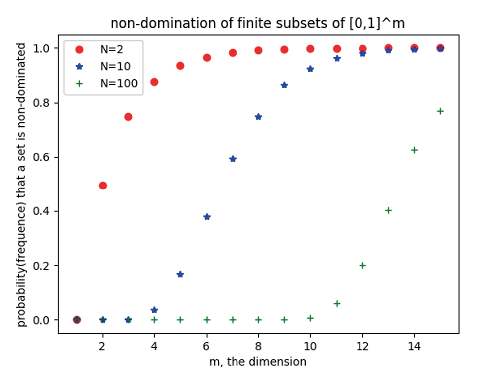
\includegraphics{figure}
	%
	% If not, use
	%\picplace{5cm}{2cm} % Give the correct figure height and width in cm
	%
	\caption{Please write your figure caption here}
	\label{fig:2}       % Give a unique label
\end{figure}

\runinhead{Run-in Heading Boldface Version} Use the \LaTeX\ automatism for all your cross-references and citations as has already been described in Sect.~\ref{sec:2}.

\subruninhead{Run-in Heading Boldface and Italic Version} Use the \LaTeX\ automatism for all your cross-refer\-ences and citations as has already been described in Sect.~\ref{sec:2}\index{paragraph}.

\subsubruninhead{Run-in Heading Displayed Version} Use the \LaTeX\ automatism for all your cross-refer\-ences and citations as has already been described in Sect.~\ref{sec:2}\index{paragraph}.
% Use the \index{} command to code your index words
%
% For tables use
%
\begin{table}[!t]
	\caption{Please write your table caption here}
	\label{tab:1}       % Give a unique label
	%
	% For LaTeX tables use
	%
	\begin{tabular}{p{2cm}p{2.4cm}p{2cm}p{4.9cm}}
		\hline\noalign{\smallskip}
		Classes     & Subclass & Length      & Action Mechanism                      \\
		\noalign{\smallskip}\svhline\noalign{\smallskip}
		Translation & mRNA$^a$ & 22 (19--25) & Translation repression, mRNA cleavage \\
		\noalign{\smallskip}\hline\noalign{\smallskip}
	\end{tabular}
	$^a$ Table foot note (with superscript)
\end{table}
%
\section{Contenido principal y organización}
\label{sec:3}
% Always give a unique label
% and use \ref{<label>} for cross-references
% and \cite{<label>} for bibliographic references
% use \sectionmark{}
% to alter or adjust the section heading in the running head
Instead of simply listing headings of different levels we recommend to let every heading be followed by at least a short passage of text. Furtheron please use the \LaTeX\ automatism for all your cross-references and citations as has already been described in Sect.~\ref{sec:2}.

If you want to list definitions or the like we recommend to use the Springer-enhanced \verb|description| environment -- it will automatically render Springer's preferred layout.

\begin{description}[Type 1]
	\item[Type 1]{That addresses central themes pertainng to migration, health, and disease. In Sect.~\ref{sec:1}, Wilson discusses the role of human migration in infectious disease distributions and patterns.}
	\item[Type 2]{That addresses central themes pertainng to migration, health, and disease. In Sect.~\ref{subsec:2}, Wilson discusses the role of human migration in infectious disease distributions and patterns.}
\end{description}

\begin{svgraybox}
	If you want to emphasize complete paragraphs of texts we recommend to use the newly defined Springer class option \verb|graybox| and the newly defined environment \verb|svgraybox|. This will produce a 15 percent screened box 'behind' your text.

	If you want to emphasize complete paragraphs of texts we recommend to use the newly defined Springer class option and environment \verb|svgraybox|. This will produce a 15 percent screened box 'behind' your text.
\end{svgraybox}

\begin{theorem}
	Theorem text goes here.
\end{theorem}

\begin{definition}
	Definition text goes here.
\end{definition}

\begin{proof}
	%\smartqed
	Proof text goes here.
	%\qed
\end{proof}

\paragraph{Paragraph Heading} %
Instead of simply listing headings of different levels we recommend to let every heading be followed by at least a short passage of text. Furtheron please use the \LaTeX\ automatism for all your cross-references and citations as has already been described in Sect.~\ref{sec:2}.

\begin{trailer}{Trailer Head}
	If you want to emphasize complete paragraphs of texts in a \verb|Trailer Head| we recommend to
	use  \begin{verbatim}\begin{trailer}{Trailer Head}
...
\end{trailer}\end{verbatim}
\end{trailer}
%
\begin{questype}{Questions}
	If you want to emphasize complete paragraphs of texts in an \verb|Questions| we recommend to
	use  \begin{verbatim}\begin{questype}{Questions}
...
\end{questype}\end{verbatim}
\end{questype}
%
%
\begin{important}{Important}
	If you want to emphasize complete paragraphs of texts in an \verb|Important| we recommend to
	use  \begin{verbatim}\begin{important}{Important}
...
\end{important}\end{verbatim}
\end{important}
%
\clearpage
\begin{warning}{Attention}
	If you want to emphasize complete paragraphs of texts in an \verb|Attention| we recommend to
	use  \begin{verbatim}\begin{warning}{Attention}
...
\end{warning}\end{verbatim}
\end{warning}

\begin{programcode}{Program Code}
	If you want to emphasize complete paragraphs of texts in a \verb|Program Code| we recommend to
	use

	\verb|\begin{programcode}{Program Code}|

	\verb|\begin{verbatim}...\end{verbatim}|

	\verb|\end{programcode}|

\end{programcode}
%
\begin{tips}{Tips}
	If you want to emphasize complete paragraphs of texts in a \verb|Tips| we recommend to
	use  \begin{verbatim}\begin{tips}{Tips}
...
\end{tips}\end{verbatim}
\end{tips}
%
%
\begin{overview}{Overview}
	If you want to emphasize complete paragraphs of texts in an \verb|Overview| we recommend to
	use  \begin{verbatim}\begin{overview}{Overview}
...
\end{overview}\end{verbatim}
\end{overview}
\clearpage
\begin{backgroundinformation}{Background Information}
	If you want to emphasize complete paragraphs of texts in a \verb|Background|
	\verb|Information| we recommend to
	use

	\verb|\begin{backgroundinformation}{Background Information}|

	\verb|...|

	\verb|\end{backgroundinformation}|
\end{backgroundinformation}
\begin{legaltext}{Legal Text}
	If you want to emphasize complete paragraphs of texts in a \verb|Legal Text| we recommend to
	use  \begin{verbatim}\begin{legaltext}{Legal Text}
...
\end{legaltext}\end{verbatim}
\end{legaltext}
%
\begin{acknowledgement}
	If you want to include acknowledgments of assistance and the like at the end of an individual chapter please use the \verb|acknowledgement| environment -- it will automatically render Springer's preferred layout.
\end{acknowledgement}

\chapter{Leyes de conservación hiperbólicas escalares}

\begin{equation}
	\difcp{U}{t}+
	\difcp{f\left(U\right)}{x}=
	0.
\end{equation}
donde $U$ es la función desconocida y $f$ es la función flujo.

\section*{Modelo de flujo de tráfico}

\begin{equation}
	\difcp{U}{t}+
	\difcp{V_{\text{max}}U\left(1-U\right)}{x}=
	0.
\end{equation}

\section*{Recuperación mejorada de petróleo}

\begin{equation}
	\difcp{S^{\text{oil}}}{t}+
	\difcp{
		\frac{q\left(S^{\text{oil}}\right)^{2}}{\left(S^{\text{oil}}\right)^{2}+\left(1-S^{\text{oil}}\right)^{2}}
	}{x}=
	0.
\end{equation}

\section*{Condición de salto de Rankine-Hugoniot}

\section*{Solución al problema de Riemann}

Una función
$U\in L^{\infty}\left(\mathbb{R}\times\mathbb{R}_{+}\right)$
es una solución entrópica


\section{Problema de Riemann}
\section{Solución débil}
\section{Función entrópica}
\section{Condición de Rankine-Hugoniot}
\section{Teorema de Lax-Wendroff}

\chapter{Método de Volúmenes Finitos}

\section*{Apéndice}
\addcontentsline{toc}{section}{Apéndice}
%
When placed at se \textit{do not} use the \verb|appendix| command when

\begin{equation}
	a \times b = c
\end{equation}
% % Problems or Exercises should be sorted chapterwise
% \section*{Problemas}
% \addcontentsline{toc}{section}{Problemas}
% %
% % Use the following environment.
% % Don't forget to label each problem;
% % the label is needed for the solutions' environment
% \begin{prob}
%     \label{prob1}
%     A given problem or Excercise is described here. The
%     problem is described here. The problem is described here.
% \end{prob}

% \begin{prob}
%     \label{prob2}
%     \textbf{Problem Heading}\\
%     (a) The first part of the problem is described here.
% \end{prob}

\nocite{*}
\printbibliography[title={Referencias},heading=bibintoc]

% %%%%%%%%%%%%%%%%%%%%% appendix.tex %%%%%%%%%%%%%%%%%%%%%%%%%%%%%%%%%
%
% sample appendix
%
% Use this file as a template for your own input.
%
%%%%%%%%%%%%%%%%%%%%%%%% Springer-Verlag %%%%%%%%%%%%%%%%%%%%%%%%%%

\appendix
\motto{All's well that ends well}
\chapter{Chapter Heading}
\label{introA} % Always give a unique label
% use \chaptermark{}
% to alter or adjust the chapter heading in the running head

Use the template \emph{appendix.tex} together with the Springer document class SVMono (monograph-type books) or SVMult (edited books) to style appendix of your book.


\section{Section Heading}
\label{sec:A1}
% Always give a unique label
% and use \ref{<label>} for cross-references
% and \cite{<label>} for bibliographic references
% use \sectionmark{}
% to alter or adjust the section heading in the running head
Instead of simply listing headings of different levels we recommend to let every heading be followed by at least a short passage of text. Furtheron please use the \LaTeX\ automatism for all your cross-references and citations.


\subsection{Subsection Heading}
\label{sec:A2}
Instead of simply listing headings of different levels we recommend to let every heading be followed by at least a short passage of text. Furtheron please use the \LaTeX\ automatism for all your cross-references and citations as has already been described in Sect.~\ref{sec:A1}.

For multiline equations we recommend to use the \verb|eqnarray| environment.
\begin{eqnarray}
\vec{a}\times\vec{b}=\vec{c} \nonumber\\
\vec{a}\times\vec{b}=\vec{c}
\label{eq:A01}
\end{eqnarray}

\subsubsection{Subsubsection Heading}
Instead of simply listing headings of different levels we recommend to let every heading be followed by at least a short passage of text. Furtheron please use the \LaTeX\ automatism for all your cross-references and citations as has already been described in Sect.~\ref{sec:A2}.

Please note that the first line of text that follows a heading is not indented, whereas the first lines of all subsequent paragraphs are.

% For figures use
%
\begin{figure}[t]
\sidecaption[t]
%\centering
% Use the relevant command for your figure-insertion program
% to insert the figure file.
% For example, with the option graphics use
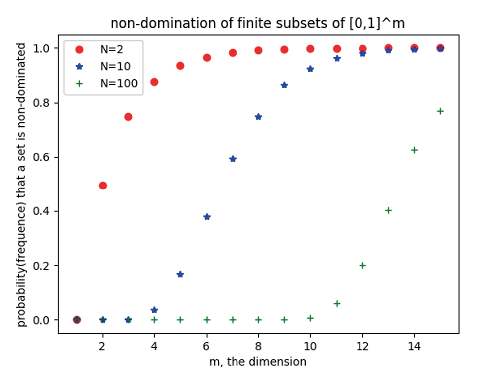
\includegraphics{figure}
%
% If not, use
%\picplace{5cm}{2cm} % Give the correct figure height and width in cm
%
\caption{Please write your figure caption here}
\label{fig:A1}       % Give a unique label
\end{figure}

% For tables use
%
\begin{table}
\caption{Please write your table caption here}
\label{tab:A1}       % Give a unique label
%
% For LaTeX tables use
%
\begin{tabular}{p{2cm}p{2.4cm}p{2cm}p{4.9cm}}
\hline\noalign{\smallskip}
Classes & Subclass & Length & Action Mechanism  \\
\noalign{\smallskip}\hline\noalign{\smallskip}
Translation & mRNA$^a$  & 22 (19--25) & Translation repression, mRNA cleavage\\
Translation & mRNA cleavage & 21 & mRNA cleavage\\
Translation & mRNA  & 21--22 & mRNA cleavage\\
Translation & mRNA  & 24--26 & Histone and DNA Modification\\
\noalign{\smallskip}\hline\noalign{\smallskip}
\end{tabular}
$^a$ Table foot note (with superscript)
\end{table}
%


\backmatter
% %%%%%%%%%%%%%%%%%%%%%%acronym.tex%%%%%%%%%%%%%%%%%%%%%%%%%%%%%%%%%%%%%%%%%
% sample list of acronyms
%
% Use this file as a template for your own input.
%
%%%%%%%%%%%%%%%%%%%%%%%% Springer %%%%%%%%%%%%%%%%%%%%%%%%%%

\Extrachap{Glosario}


Use the template \emph{glossary.tex} together with the Springer document class SVMono (monograph-type books) or SVMult (edited books) to style your glossary\index{glossary} in the Springer layout.


\runinhead{glossary term} Write here the description of the glossary term. Write here the description of the glossary term. Write here the description of the glossary term.
% 
\Extrachap{Soluciones}

\section*{Problemas del Capítulo~\ref{intro}}

\begin{sol}{prob1}
The solution\index{problems}\index{solutions} is revealed here.
\end{sol}


\begin{sol}{prob2}
\textbf{Problem Heading}\\
(a) The solution of first part is revealed here.\\
(b) The solution of second part is revealed here.
\end{sol}


\printindex
\end{document}
